\documentclass[../main.tex]{subfiles}

\begin{document}

\chapter[Temperature and Ice]{The Impact of Temperature on Antarctic Ice}

The variable which we found had the largest impact on the behaviour of ice in Antarctica is temperature. This follows naturally from the basic thermodynamics of phase change. As the temperature increases we see lower concentrations of sea ice, and as the temperature increases we see lower concentrations of sea ice. The extent of this relationship will be explored in detail in this chapter. We will first look at the relationship through density plots \textcolor{red}{Check name of plots}. Before calculating correlations and looking at the similarities and differences of the two different variables.

For the purpose of this chapter, when we use temperature we will use skin temperature as discussed before \textcolor{red}{Write up different temperatures.}


\section{Visually comparing Temperature and Ice}
Before we get into any aggregation let's compare the amount of ice at each time and space coordinate in our dataset with the temperature at the associated grid point. 

\begin{figure}[h!]
    \centering
    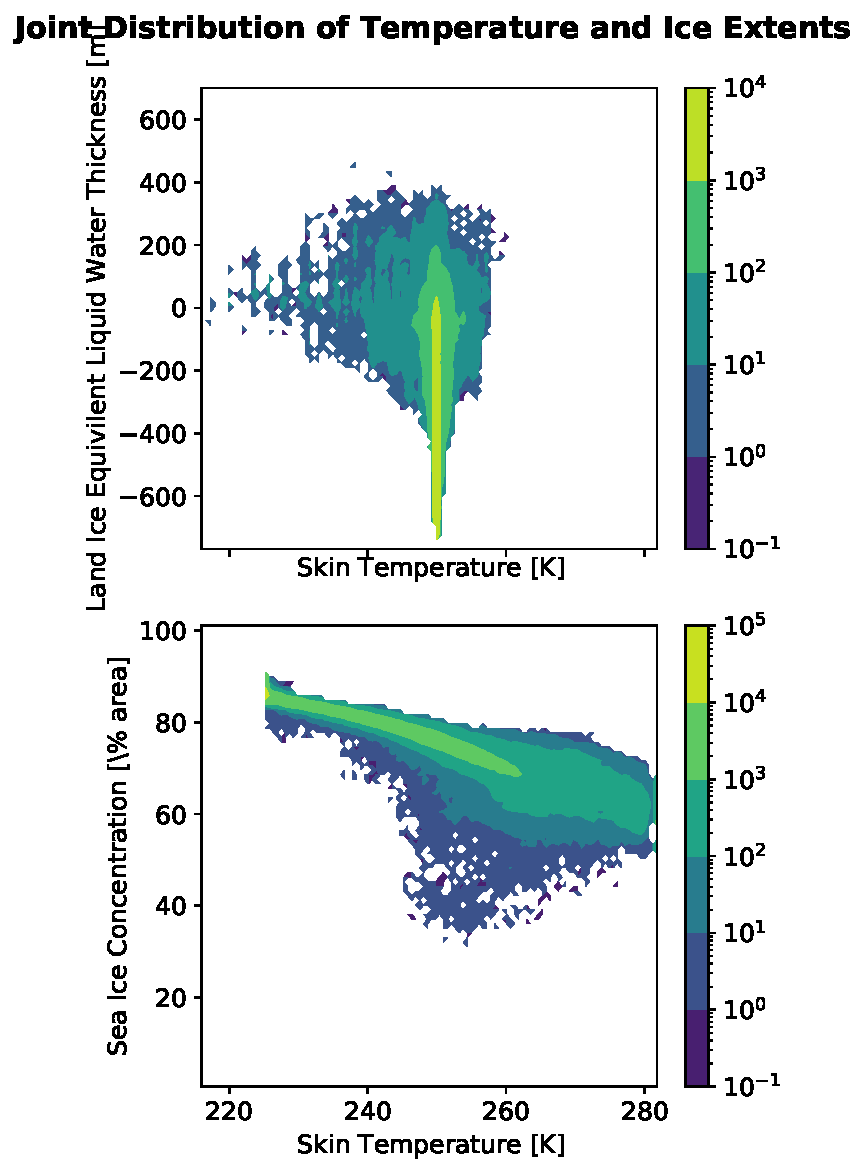
\includegraphics{images/week8/hres/distribution_of_temperature_ice}
    \caption{Distribution of skin temperature against ice. This is a 2 dimensional histogram where the colour represents the number of points in our dataset with a given temperature and amount of ice. The top subplot contains all the gridpoints over land, and the bottom subplot contains all the gridpoints over the sea.}
    \label{fig:joint_distribuition_temp_ice}
\end{figure}

This plot (Figure \ref{fig:joint_distribuition_temp_ice}) tells us an interesting story. For sea ice, we can observe a significant relationship between skin temperature and SIC. This relationship matches with our intuition, which is great. However land ice doesn't exhibit the same strong relationship as sea ice. This is interesting as it suggests that it is driven by a different set of processes. We will have to be careful about this in our ongoing analysis.

One thing we need to remember with this plot is that it will be exhibiting some spatial bias because some locations will have higher values of ice and lower temperatures. Additionally these plots only contain data points from 2002 because the land ice data only 

\begin{figure}[h!]
    \centering
    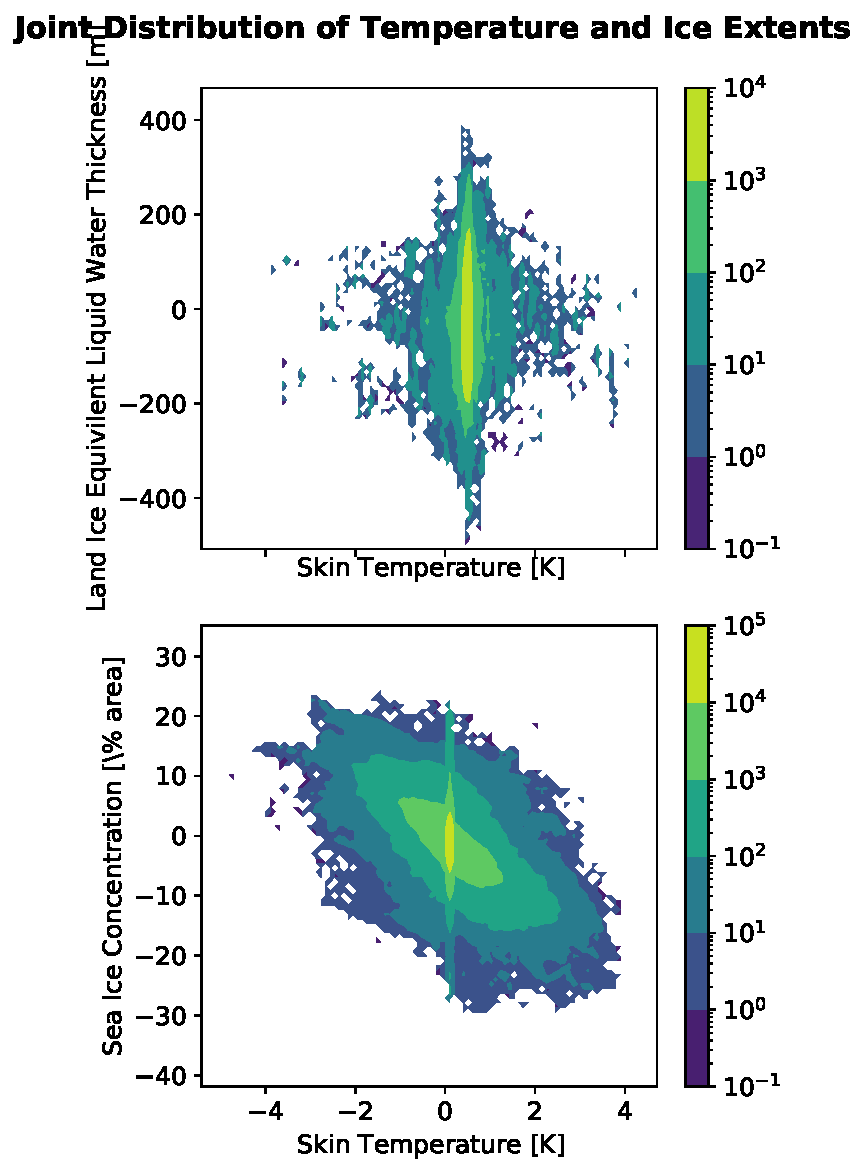
\includegraphics{images/week8/hres/distribution_of_temperature_ice_anomalous}
    \caption{Distribution of anomalous  skin temperature against anomalous ice. This is a 2 dimensional histogram where the colour represents the number of points in our dataset with a given temperature and amount of ice. The top subplot contains all the gridpoints over land, and the bottom subplot contains all the gridpoints over the sea.}
    \label{fig:joint_distribuition_temp_ice}
\end{figure}

\section*{Things still to do for this section}
\begin{enumerate}
    \item Add to the scatter plots
    \begin{itemize}
        \item Trend lines.
        \item Statistics such as correlations
        \item normalised colour-bars
        \item Make into a 4 panel design
    \end{itemize}
    \item Regress temperature onto ice.
    \item Plot mean values for ice and temperature to explain removing the anomalies.
    \item Fill out red citation notes in the text.
\end{enumerate}

\end{document}